%! Author = Daniel Schäfer
%! Date = 03.11.2023

% Preamble
\documentclass[12pt, a4paper, ngerman, bibliography=totocnumbered]{article}

% Packages
\usepackage{amsmath}
\usepackage[utf8]{inputenc}
%\usepackage[sfdefault]{roboto}
\usepackage[T1]{fontenc}
\usepackage{lmodern}
\usepackage{graphicx}
\usepackage{babel}
\usepackage[hidelinks]{hyperref}
\usepackage[table]{xcolor}
\usepackage{float}
\usepackage[top=1in, bottom=2cm, includefoot]{geometry}
\usepackage{wrapfig}
\usepackage{color}
\usepackage{minted}
\usepackage{listings}
\usepackage{caption}
\usepackage{awesomebox}
\usepackage{csquotes}
\usepackage{makecell}
\usepackage{datetime}
% \usepackage{background}
\usepackage{nameref}
\usepackage{tocbibind}
\usepackage{tocloft}
\usepackage{amsmath}
\usepackage{hyphenat}
\usepackage{siunitx}
\usepackage{todonotes}
\usepackage{orcidlink}

\sisetup{per-mode=symbol}
\sisetup{output-decimal-marker = {,}}

\numberwithin{equation}{section}

\setlength{\cftbeforesecskip}{8pt}

\newdateformat{versiondateformat}{\THEDAY.\THEMONTH}

\renewcommand{\fcolorbox}[4][]{#4}
\renewcommand{\arraystretch}{1.5}

\graphicspath{{assets/}}

\addto{\captionsngerman}{\renewcommand{\refname}{Literaturverzeichnis}}
\renewcommand\listoflistingscaption{Quellcodeverzeichnis}
\renewcommand{\listingscaption}{Codeblock}

\DeclareCaptionFormat{custom}
{
    \centering \textbf{\small #1#2}\textit{\small #3}
}

\DeclareUnicodeCharacter{2014}{\dash}

\captionsetup{format=custom}

\setlength{\tabcolsep}{8pt}
\renewcommand{\arraystretch}{1.5}

\newcommand{\ohm}{\Omega}

\newcommand{\itemwithdesc}[2]{\textbf{#1}\\ \vspace*{-3mm}\\ \hspace*{5mm} \begin{minipage}{.9\linewidth}#2\end{minipage} \vspace*{2mm}}

\newcommand{\version}{\versiondateformat\today}
\newcommand{\newPar}{\newline\newline}

\newcommand{\gq}[1]{\glqq{}#1\grqq{}}
\newcommand{\zB}{z.\,B.}
\newcommand{\imageref}[1]{\textit{\hyperref[#1]{Abbildung} \ref{#1}}}

% \backgroundsetup{contents={Entwurf-\version}, scale=3, opacity=0.6, color=gray, angle=0, vshift=-131pt}

\title{\projekttitle}

% Keine Einrückung
\setlength\parindent{0pt}

% Document
\begin{document}
    \pagenumbering{gobble}
    %! Author = Daniel Schäfer
%! Date = 01.11.2023

\begin{titlepage}

    % Header
    \noindent\begin{minipage}{50mm}
         
\includegraphics[width=\linewidth]{thm}
    \end{minipage}
    \hfill
    \begin{minipage}{50mm}
        {\raggedleft Fakultät für Informatik \par}
    \end{minipage}
    \vspace*{2cm}

    % Titel
    \begin{center}
    \vspace{55mm}

    {\LARGE \bfseries Implementierung einer\\Echtzeit-Bilderkennung und Steuerung\\basierend auf einem selbsttrainierten\\Modell mit YOLO und einem\\TurtleBot3-Roboter\\}

    \vspace{28mm}

    {\large{Master-Wahlmodul}} \\[2mm]

    {\Large{\bfseries Autonome Mobile Roboter}} \\[2mm]

    {\Large{Sommersemester 2025}} \\[9mm]

    {\large{Prof. Dr. Thomas Ihme}}\\[8mm]

    \vfill
    {\large{verfasst von}}\\
    {\large{\bfseries Ann-Kathrin Stracke \orcidlink{0009-0009-9146-9069}}}\\
    {\large{\bfseries Daniel Schäfer \orcidlink{0009-0002-8754-6999}}}\\

    {\small{\today}}
    \end{center}

\end{titlepage}

    \section*{Abstract}
In dieser Arbeit wurde ein System zur Echtzeit-Bilderkennung und autonomen Steuerung eines TurtleBot3-Roboters entwickelt. 
Ziel war es, ein eigenes Objekterkennungsmodell auf Basis des Bildverarbeitungsframeworks YOLO zu trainieren und dieses so in das Robot Operating System~2 (ROS~2) zu integrieren, 
dass der Roboter im konkreten Beispiel Richtungspfeile erkennt und entsprechend reagiert. 
Das Projekt vereint zentrale Aspekte aus den Bereichen Robotik, Bildverarbeitung und künstlicher Intelligenz und wurde vollständig praktisch umgesetzt.
\newPar
Ein wesentlicher Bestandteil war die Erstellung eines Trainingsdatensatzes, der hunderte Bilder mit verschiedenen Pfeilformen und -farben enthielt. 
Nach dem Labeling der Daten wurde das YOLO-Modell mithilfe von PyTorch auf einem leistungsfähigen Rechner mit GPU trainiert. 
Das daraus entstandene Modell konnte anschließend in das Robotersystem eingebunden werden. 
Über eine Kamera, die am TurtleBot3 montiert wurde, werden kontinuierlich Bilder aufgenommen, die das Modell auswertet. 
Anhand der erkannten Objekte entscheidet das System, ob der Roboter nach links, rechts oder geradeaus fahren soll.
\newPar
Neben der technischen Umsetzung lagen die Herausforderungen vor allem in der Einarbeitung in ROS~2, der Einbindung der Kamera sowie der Synchronisation zwischen Trainingsumgebung und Roboter. 
Trotz dieser Hürden konnte ein stabiles und funktionales Gesamtsystem realisiert werden, das zeigt, wie moderne KI-Verfahren sinnvoll mit mobiler Robotik kombiniert werden können.
    \newpage

    \tableofcontents
    \newpage
    \pagenumbering{arabic}

    \section{Einleitung}\label{sec:einleitung}
Im Zuge der fortschreitenden Digitalisierung und Automatisierung gewinnen mobile Robotersysteme zunehmend an Bedeutung. 
Insbesondere im Bereich der autonomen Navigation und Echtzeit-Umgebungswahrnehmung eröffnen sich durch den Einsatz moderner Sensortechnik und künstlicher Intelligenz neue Anwendungsmöglichkeiten. 
Diese Entwicklungen stellen jedoch nicht nur technische Herausforderungen dar, sondern erfordern auch ein fundiertes Verständnis für die zugrunde liegenden Technologien und deren Zusammenspiel.
\newPar
Die vorliegende Projektarbeit widmet sich dem Aufbau und der praktischen Umsetzung eines solchen Robotersystems auf Basis des TurtleBot3. 
Im Fokus steht dabei die Integration eines auf Deep Learning basierenden Objekterkennungsmodells (YOLO) in ein mit dem Robot Operating System 2 (ROS 2) gesteuertes System. 
Die Kombination dieser beiden Technologien erlaubt die Entwicklung eines autonomen Roboters, der visuelle Reize in seiner Umgebung interpretieren und darauf in Form von gezielten Bewegungen reagieren kann.
\newPar
Die Arbeit verfolgt damit einen Ansatz, der Kenntnisse aus den Bereichen Robotik, Softwareentwicklung, Bildverarbeitung und künstliche Intelligenz zusammenführt. 
Durch den starken Praxisbezug soll zum einen ein funktionales System entstehen, als auch ein tieferes Verständnis für die Herausforderungen und Möglichkeiten moderner mobiler Robotik erlangt werden.
\subsection{Motivation}
Die Motivation für die vorliegende Arbeit ist es, theoretisches Wissen mit praktischer Erfahrung zu verknüpfen und einen Einblick in die komplexe Welt mobiler Robotiksysteme zu gewinnen.
Ein zentrales Lernziel des Projekts ist die Einarbeitung in das Robot Operating System 2 (ROS 2), das für viele moderne Robotik-Anwendungen als technologische Basis dient. 
Da die Projektgruppe bislang keine praktischen Erfahrungen mit ROS 2 gesammelt hat, ist eine gründliche Auseinandersetzung mit dessen Architektur, Kommunikationsprinzipien und Konfigurationsmöglichkeiten erforderlich. 
Im Vergleich zu anderen Entwicklungsumgebungen gilt ROS 2 als besonders leistungsfähig, bringt jedoch auch eine hohe Komplexität mit sich, die gerade für Einsteiger eine steile Lernkurve bedeutet. 
Bereits die Installation, Inbetriebnahme und das Verständnis der systeminternen Abläufe stellen eine Herausforderung dar.
Diese Einarbeitungsphase bildet die technische Grundlage für die spätere Steuerung des TurtleBot3 und ist somit ein wesentlicher Bestandteil der Arbeit.
\newPar
Darüber hinaus möchte sich die Projektgruppe intensiv mit Methoden der Bildverarbeitung und dem Einsatz künstlicher Intelligenz in der Robotik beschäftigen. 
Ziel ist es, ein fundiertes Verständnis für das YOLO-Framework zur Objekterkennung zu entwickeln und dessen praktische Anwendung im Zusammenspiel mit ROS 2 zu erproben. 
Um gezielt Wissen im Bereich des Trainings von KI-Modellen zu erwerben, soll zudem ein bestehendes YOLO-Modell weitertrainiert und auf spezifische Erkennungsobjekte angepasst werden.
Die Kombination beider Technologien stellt eine anspruchsvolle, aber zugleich äußerst lehrreiche Herausforderung dar, die es ermöglicht, ein praxisnahes Projekt umzusetzen.
    \section{Konzept}\label{sec:konzept}
Ziel dieser Arbeit ist die Entwicklung eines Systems zur Echtzeit-Bilderkennung und -Steuerung eines TurtleBot3-Roboters unter Verwendung eines selbst trainierten YOLO-Modells. 
Dabei soll ein praxisnaher Einblick in das Training und den Einsatz künstlicher Intelligenz im Bereich der mobilen Robotik gewonnen werden. 
Das trainierte Modell soll aufgrund der erhöhten Rechenanforderungen auf einem separaten Rechner mit GPU ausgeführt werden, während der Roboter über ROS 2 Kamera- und Steuerdaten mit dem Rechner austauscht. 
Zur Demonstration der Funktionalität sollen Richtungspfeile als Erkennungsobjekte verwendet werden. 
Erkennt das System einen Pfeil, soll der Roboter entsprechend abbiegen.
Dieses Szenario ermöglicht einen gezielten Einblick in die Objekterkennung und die Verwendung von ROS.
\newPar
Speziell zur Anwendung kommen soll das Bildverarbeitungsframework YOLO, das mit einer Vielzahl von vortrainierten Objektklassen bereits eine gute Basis zur Objekterkennung bietet.
Dieses kann mittels Tools des Herstellers Ultralytics bzw. der Open\hyp{}Source\hyp{}Bibliothek PyTorch speziell nachtrainiert werden, um eigene benutzerdefinierte Objekte erkennen zu können.
    \section{Grundlagen}
Für das Verständnis der im Projekt eingesetzten Technologien und deren Zusammenspiel ist es notwendig, zunächst die zugrunde liegenden technischen Komponenten und Frameworks näher zu erläutern. 
Dieses Kapitel stellt die wesentlichen Grundlagen vor, die für die Entwicklung des Systems relevant sind. 
Dazu zählen sowohl die verwendete Hardwareplattform in Form des TurtleBot3 als auch das Software-Framework ROS 2, das als zentrale Entwicklungsumgebung dient. 
\subsection{Turtlebot3}
Der TurtleBot3 ist ein kompakter, kostengünstiger und modular erweiterbarer mobiler Roboter, der auf dem Robot Operating System (ROS) basiert. 
Er wurde für Anwendungen in den Bereichen Forschung, Lehre, Prototypenentwicklung sowie für den hobbymäßigen Robotik-Einsatz konzipiert. 
Ziel des Turtlebot3 ist es, eine robuste, funktionsreiche und zugleich leicht zugängliche Lösung bereitzustellen, die sowohl in akademischen als auch industriellen Kontexten einsetzbar ist.
\cite{tb3_overview}\cite{tb3_home}
\newPar
Der Aufbau des TurtleBot3 ist in \imageref{tb3_components} veranschaulicht.
Als zentrale Recheneinheit verwendet der TurtleBot3 einen Raspberry Pi 4, einen leistungsfähigen und weit verbreiteten Einplatinencomputer (SBC).
Zur Umgebungswahrnehmung ist der Roboter mit einem 360°-LiDAR-Sensor ausgestattet, der präzise Abstandsmessungen und Kartierung ermöglicht. 
Darüber hinaus sind verschiedene optionale Sensoren wie Ultraschall- oder Infrarotsensoren integrierbar. 
Die mechanische Plattform ist modular aufgebaut und besteht aus leichtgewichtigen, teilweise 3D-gedruckten Komponenten, die eine einfache Anpassung und Erweiterung ermöglichen.
Das in dieser Arbeit verwendete TurtleBot3 Burger-Modell hat eine Größe von etwa \SI{14}{\centi\meter}~$\times$~\SI{18}{\centi\meter}~$\times$~\SI{19}{\centi\meter} und zeichnet sich zusätzlich durch eine maximale Geschwindigkeit von \SI{0,22}{\meter\per\second} aus.
\cite{tb3_specifications}\cite{tb3_overview}
\newPar
\begin{figure}[H]
    \centering
    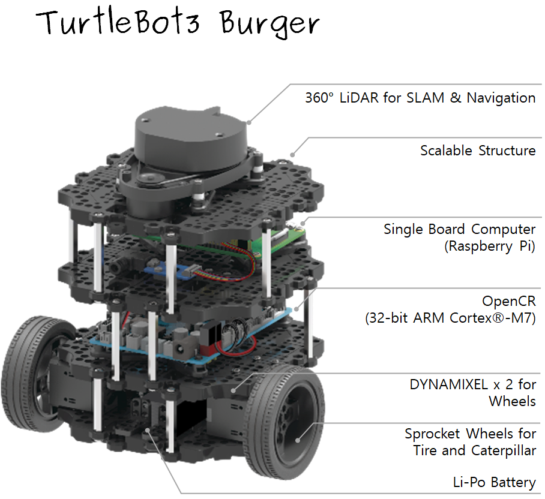
\includegraphics[width=10cm]{turtlebot3_burger_components}
    \caption{Turtlebot3 Burger Komponenten \cite{tb3_specifications}}\label{tb3_components}
\end{figure}
Technologisch unterstützt der TurtleBot3 zentrale Funktionen wie Simultaneous Localization and Mapping (SLAM) und autonome Navigation, wodurch der Roboter in der Lage ist, Umgebungen selbstständig zu kartieren und sich sicher darin zu bewegen. 
Die Steuerung kann über diverse Schnittstellen erfolgen, beispielsweise durch einen Laptop, ein Gamepad oder Android-basierte Endgeräte, was eine flexible Bedienung ermöglicht.
Zur mobilen und kabellosen Nutzung erfolgt die Energieversorgung über einen LiPo-Akku mit 1.800 mAh.
\cite{tb3_home}\cite{tb3_specifications}
\newPar
Da der Turtlebot3 von sich aus nicht über eine Kamera verfügt, wurde diese nachträglich am Roboter angebracht. 
Im Projekt wird zur Aufnahme eine Raspberry Pi Camera 1.3 verwendet.
Diese 5-Megapixel-Kamera mit festem Fokus kann Bilder mit einer Auflösung von bis zu 2592x1944 Pixeln aufnehmen. 
Sie unterstützt Videoaufnahmen in 1080p bei 30 Bildern pro Sekunde, 720p bei 60 Bildern pro Sekunde sowie 640x480p bei bis zu 90 Bildern pro Sekunde.
Während des Projekts wurde die Auflösung von 640x480 Pixeln verwendet, um ein möglichst flüssiges Bild zu erhalten und um die später benötigte Rechenleistung zu minimieren.
\cite{pi_camera}
\subsection{ROS 2}
Zur Steuerung und zum Auslesen der Sensoren des Turtlebot3 wird in dieser Arbeit das Robot Operation System 2 (ROS 2) in der Version Humble Hawksbill verwendet. 
Für diese Version wurde sich entschieden, da zum Start des Projekts auf dem Raspberry Pi bereits Ubuntu 22.04 mit ROS 2 Humble installiert war.
\newPar
ROS 2 ist ein Framework zur Entwicklung verteilter Softwaresysteme für Robotikanwendungen. 
Es bietet Werkzeuge, Bibliotheken und Konventionen zur Entwicklung modularer, skalierbarer und wiederverwendbarer Komponenten. 
ROS 2 folgt einem dezentralen Architekturansatz, bei dem Softwarebausteine als unabhängige Prozesse (sogenannte Nodes) organisiert sind, die über verschiedene Kommunikationsmechanismen Daten austauschen können.
Topics sind in ROS 2 das zentrale Konzept für die asynchrone, publish-subscribe-basierte Kommunikation zwischen Nodes. 
Ein Node kann Daten zu einem Topic veröffentlichen (publish), während andere Nodes diese Daten abonnieren (subscribe). 
Die Kommunikation erfolgt einseitig und ist ideal für kontinuierliche Datenströme wie Sensordaten, Statusinformationen oder Steuerbefehle.
\cite{ros2_documentation}\cite{ros2_nodes}\cite{ros2_topics}
\newPar
Ein wesentlicher Vorteil von ROS 2 besteht in der großen Anzahl bereits verfügbarer Softwarepakete (Packages), die viele häufig benötigte Funktionalitäten abdecken. 
Dazu zählen unter anderem Pakete zur Ansteuerung von Sensoren, Kameras und Motoren sowie Module für Lokalisierung, Pfadplanung oder Visualisierung. 
Diese vorgefertigten Komponenten ermöglichen eine erhebliche Reduktion des Entwicklungsaufwands und erlauben es, sich auf projektspezifische Erweiterungen zu konzentrieren, statt grundlegende Funktionen selbst implementieren zu müssen.
\subsection{YOLO}
YOLO steht für \gq{You Only Look Once} und ist ein modernes Framework und Modell zur Objekterkennung in Bildern und Videos. 
Im Gegensatz zu früheren Ansätzen, bei denen Objekte zunächst lokalisiert und anschließend klassifiziert wurden, verfolgt YOLO einen sogenannten \gq{Single Shot}-Ansatz. 
Das bedeutet, dass das gesamte Bild in einem einzigen Durchlauf analysiert wird. 
Dabei erkennt das Modell gleichzeitig, welche Objekte sich im Bild befinden, wo sie sich befinden (über sogenannte Bounding Boxes) und welcher Klasse sie angehören. 
Dieses Verfahren ist besonders effizient und eignet sich daher sehr gut für Echtzeitanwendungen und daher auch speziell für (autonome) Robotik-Projekte.
\newPar
Ein wichtiges Unterscheidungsmerkmal bei der Arbeit mit bildverarbeitenden Modellen ist die Abgrenzung zwischen Bildklassifikation, Objekterkennung und Segmentierung: 
\begin{itemize}
\item 
Bei der Klassifikation wird einem gesamten Bild genau eine Klasse zugewiesen. In \imageref{beispiel_klassifizierung} findet sich ein Beispiel mit einer Person, einem Stativ und einer Sicherheitsweste.

\item
Bei der Objekterkennung wird dies spezialisiert. Sie erkennt mehrere Objekte innerhalb eines Bildes, lokalisiert diese und ordnet ihnen jeweils eine Klasse zu. 
Dies ist auch der zentrale Anwendungsbereich von YOLO. Das Beispiel in \imageref{beispiel_objekterkennung} zeigt eine erkannte Person mit mehreren Verkehrskegeln.

\item
Noch detailliertere Ergebnisse können mit der Segmentierung erziehlt werden. Dabei wird jedem Pixel im Bild eine Klasse zugewiesen wird. 
Es wird im Spezielles also auch die Form des Objektes erkannt (\imageref{beispiel_segmentierung}).

\end{itemize}

\begin{figure}[H]
    \centering
    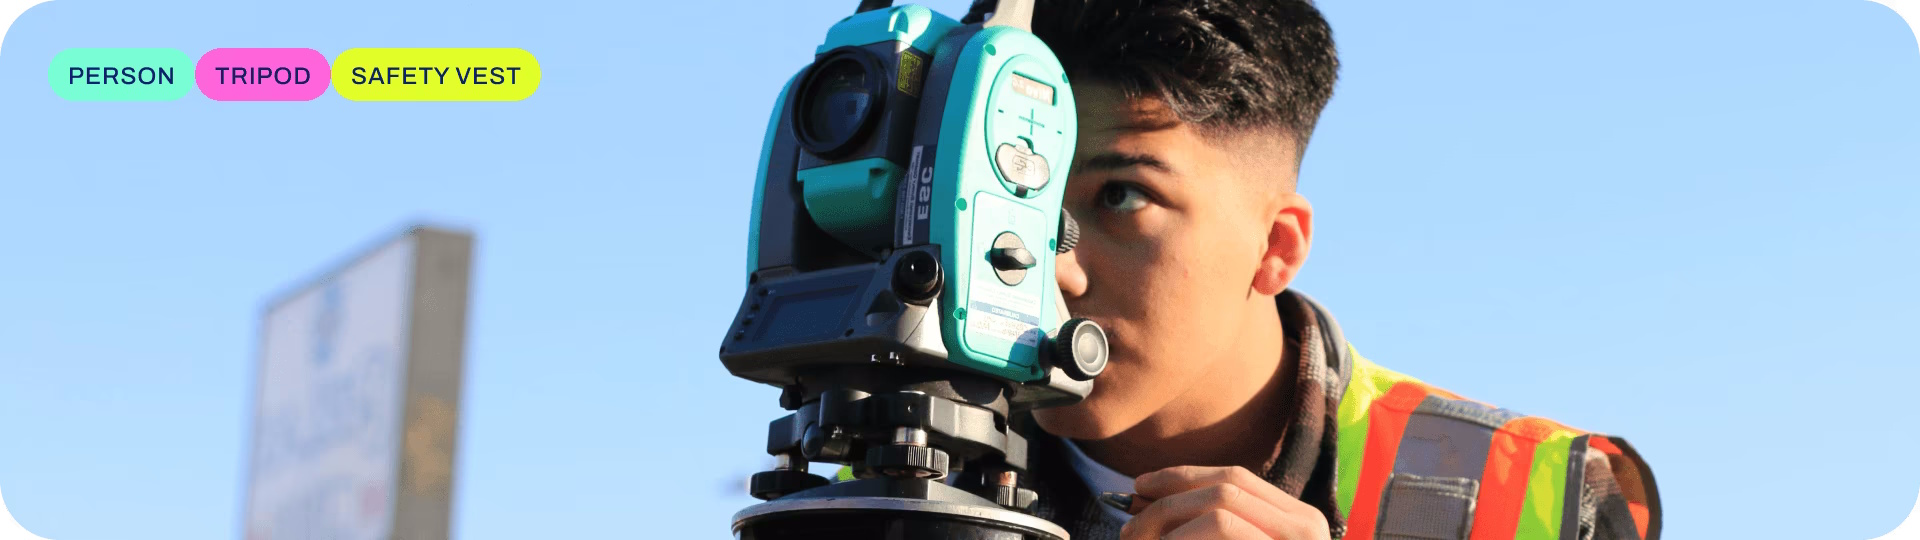
\includegraphics[width=\linewidth]{klassifizierung}
    \caption[Beispiel Klassifizierung]{Beispiel Klassifizierung (https://github.com/ultralytics/docs/releases/download/0/image-classification-examples.avif)}\label{beispiel_klassifizierung}
\end{figure}

\begin{figure}[H]
    \centering
    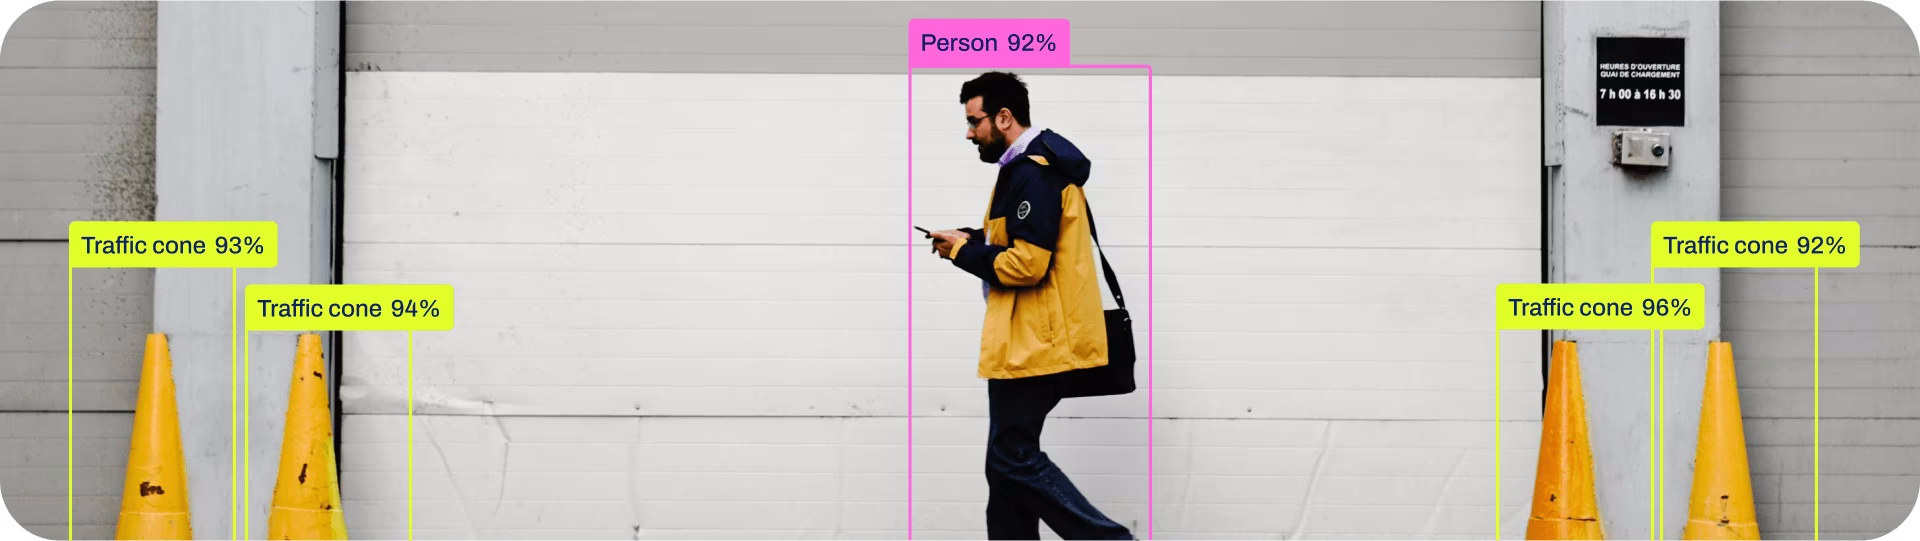
\includegraphics[width=\linewidth]{objekterkennung}
    \caption[Beispiel Objekterkennung]{Beispiel Objekterkennung (https://github.com/ultralytics/docs/releases/download/0/object-detection-examples.avif)}\label{beispiel_objekterkennung}
\end{figure}

\begin{figure}[H]
    \centering
    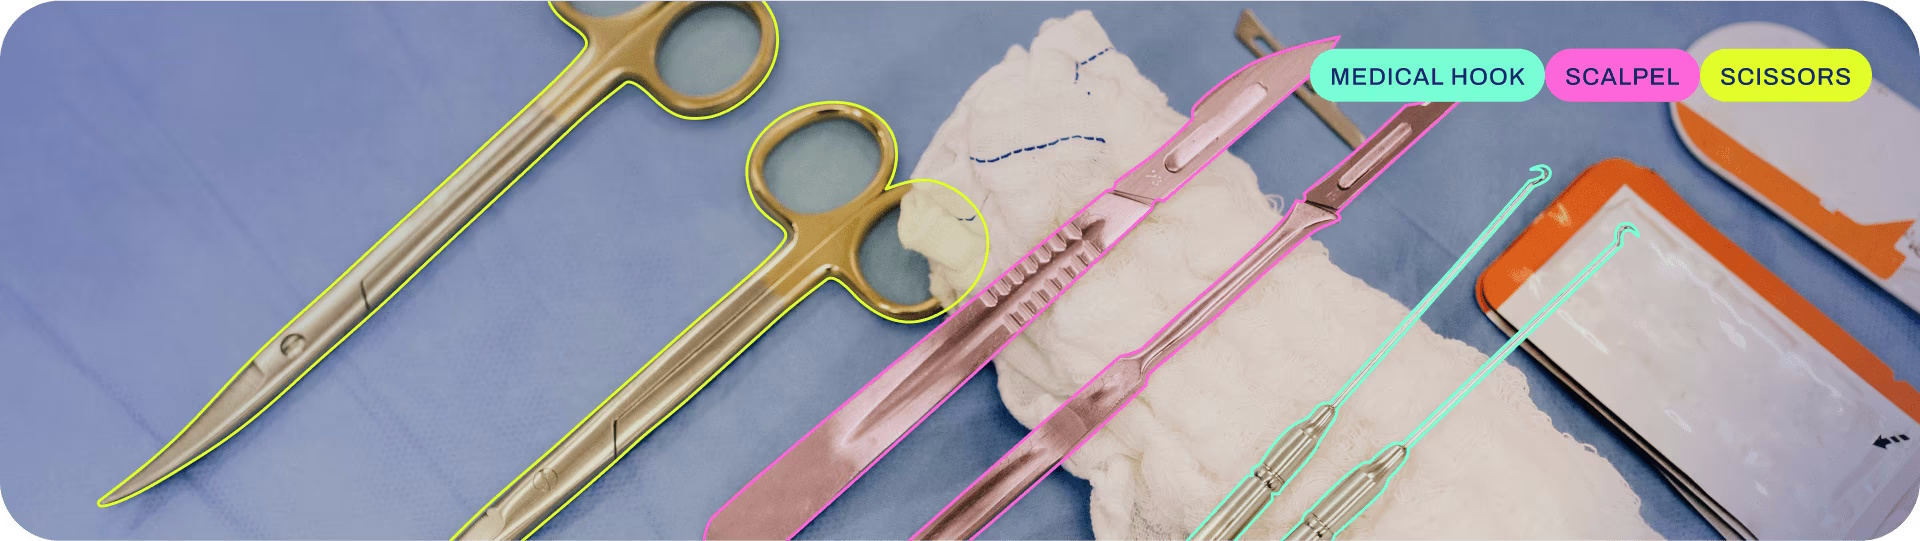
\includegraphics[width=\linewidth]{segmentierung}
    \caption[Beispiel Segmentierung]{Beispiel Segmentierung (https://github.com/ultralytics/docs/releases/download/0/instance-segmentation-examples.avif)}\label{beispiel_segmentierung}
\end{figure}

YOLO wurde seit seiner ersten Veröffentlichung kontinuierlich weiterentwickelt. 
Die frühen Versionen, wie YOLOv1 bis YOLOv3, legten den Grundstein für schnelle Erkennung. 
Ab YOLOv4 wurden weitere Optimierungen eingeführt, die vor allem das Training auf eigenen Datensätzen vereinfachten. 
Mit YOLOv5, das von der Firma Ultralytics gepflegt wird, wurde die Nutzung nochmals zugänglicher und die verschiedenen Modellgrößen wurden eingeführt.
Die Modellgrößen unterscheiden sich im Umfang der enthaltenen Parameter und bestimmen damit die Lauffähigkeit und Performance basierend auf den verfügbaren Hardwareressourcen.
Es gibt die Modellgrößen: \gq{n} (nano), \gq{s} (small), \gq{m} (medium), \gq{l} (large) und \gq{x} (extra large).
Neuere Versionen wie YOLOv6 bis YOLOv8 unterstützen neben der Objekterkennung auch Segmentierungs- und Tracking-Aufgaben.
\newPar
In diesem Projekt wurde sich für Version YOLOv11 in der Variante \gq{n} entschieden, also YOLOv11n.
Diese Modellvariante ist besonders kompakt und eignet sich dadurch gut für Anwendungen mit begrenzten Ressourcen.
Besonders ausschlaggebend für diese Entscheidung war die hohe Genauigkeit bei der Erkennung und Lokalisierung von Objekten (also bei der Berechnung der Bounding Boxes),
sowie die Performance auf ressourcenarmen Systemen, da das Training und die Inferenz zuerst innerhalb einer virtuellen Maschine durchgeführt wurde.
\newPar
Inferenz bezeichnet bei bildverarbeitenden Modellen den Prozess, bei dem ein trainiertes Modell neue, bisher unbekannte Bilddaten analysiert und daraus eine 
Vorhersage oder Entscheidung ableitet. Dabei greift das Modell auf das Wissen zurück, das es während des Trainings mit zahlreichen Beispielen (den Trainingsdaten) gelernt hat. 
Damit eine Inferenz durchgeführt werden kann, braucht es zunächst ein fertig trainiertes Modell sowie passende Eingabedaten, also ein neues Bild.
Zusätzlich ist eine geeignete Rechenumgebung notwendig. Oft wird dazu spezialisierte Hardware wie GPUs eingesetzt. da die Verarbeitung von Bilddaten rechenintensiv sein kann.
Mit passend ausgewählten und angepassten Modellen ist es jedoch auch möglich, Inferenz auf ressourcenärmeren Systeme auszuführen.
Inferenz ist damit der praktische Einsatz des zuvor gelernten Modells, etwa um Objekte zu erkennen, Bilder zu klassifizieren oder bestimmte Bildbereiche zu segmentieren.
\newPar
Die YOLO-Modelle sind bereits in der Lage, eine Vielzahl von vortrainierten Klassen zu erkennen, können aber für spezielle benutzerdefinierte Klassen nachtrainiert werden.
Genau dies ist ein Kernaspekt dieses Projektes und Basis der Entscheidung für YOLO als Modellframework.
\cite{yolo_docu}
    \clearpage
    \section{Vorbereitung}
Damit das Projekt erfolgreich umgesetzt werden kann, sind im Vorfeld mehrere technische und organisatorische Vorbereitungen erforderlich. 
Insbesondere die Einrichtung der ROS-2-Umgebung sowie die Sicherstellung einer stabilen Netzwerkverbindung zwischen dem Steuerrechner und dem TurtleBot3 stellen grundlegende Voraussetzungen für die Durchführung des Projekts dar. 
Darüber hinaus wird eine erste praktische Auseinandersetzung mit ROS 2 vorgenommen, um ein grundlegendes Verständnis der Funktionsweise und Struktur des Systems zu erlangen.
\subsection{Installation ROS 2}
Zur Herstellung einer funktionalen Kommunikationsverbindung zwischen dem Steuerrechner und dem TurtleBot3 wurde der offizielle Quick Start Guide \cite{tb3_quickstart} von Robotis herangezogen. 
Um die Kompatibilität beider Systeme sicherzustellen, wurde auf dem Rechner dieselbe Version von ROS 2 (Humble Hawksbill) installiert.
Dazu wurde zunächst eine virtuelle Maschine mit Ubuntu 22.04 eingerichtet. 
Anschließend erfolgte die Installation aller für ROS 2 relevanten Pakete sowie der Standardsoftware für den TurtleBot3, darunter Tools zur Kartografierung, Sen\-sor\-da\-ten\-er\-fass\-ung und Robotersteuerung.
\newPar
Um eine konsistente Kommunikation zu ermöglichen, wurden auf beiden Systemen spezifische Parameter vereinheitlicht: Als Modell wurde \textit{BURGER} gewählt, welches der Hardwarekonfiguration des eingesetzten TurtleBot3 entspricht. Die Domain-ID für ROS 2 wurde auf den Wert \textit{5} gesetzt, um die Kommunikation auf eine definierte Gruppe von ROS-Nodes zu beschränken. 
Zudem kam mit \textit{rmw\_fastrtps\_cpp} eine Middleware-Implementierung zum Einsatz, die auf dem DDS-Standard basiert und für die Datenübertragung zwischen ROS-2-Nodes zuständig ist.
\newPar
Darüber hinaus wurde die ROS-Installation auf dem TurtleBot vollständig neu durchgeführt, um potenzielle Konflikte mit vorherigen Installationen oder Konfigurationen auszuschließen.
\subsection{Netzwerkverbindung}
Für die bidirektionale Kommunikation zwischen dem TurtleBot3 und dem Steuerrechner war die Einbindung beider Geräte in ein gemeinsames Netzwerk erforderlich. 
In der Anfangsphase des Projekts wurde hierzu ein Smartphone-Hotspot verwendet. 
Dieser Ansatz erwies sich jedoch aufgrund erheblicher Schwankungen in der Übertragungsqualität als unzuverlässig.
\newPar
Im weiteren Verlauf wurde daher ein WLAN-Repeater eingesetzt, der ein stabiles und gemeinsames Netzwerk für beide Geräte bereitstellte. 
Zur Einbindung der Geräte in dieses Netzwerk wurden entsprechende Anpassungen an der Netzwerkkonfiguration des Turtlebots in der Datei \textit{/etc/netplan/50-cloud-init.yaml} vorgenommen und durch den Befehl \textit{sudo netplan apply} aktiviert.
Durch diese optimierte Lösung konnte eine stabile Datenübertragung sichergestellt werden, insbesondere für die Übermittlung der Bilddaten in Echtzeit.
\newPar
Sobald beide Systeme erfolgreich im Netzwerk verbunden waren, wurde die Kommunikation über das SSH-Protokoll eingerichtet. 
Dies ermöglichte den Fernzugriff auf den TurtleBot3 ohne zusätzliche Peripheriegeräte wie Bildschirm oder Tastatur, was die Handhabung im Projektalltag deutlich vereinfacht hat.
\subsection{Einarbeitung ROS 2}
Zur Überprüfung der erfolgreichen Systeminstallation wurde das vorinstallierte Teleop-Programm genutzt, mit dem sich der TurtleBot3 manuell über die Tastatur steuern lässt. 
Darüber hinaus wurde mithilfe von rqt ein erster Einblick in die Kommunikation über Topics gewonnen. 
Der Topic Monitor (\imageref{rqt}) erlaubte die Analyse von Sensordatenströmen und bot eine visuelle Darstellung aktiver Kommunikationskanäle.
\begin{figure}[H]
    \centering
    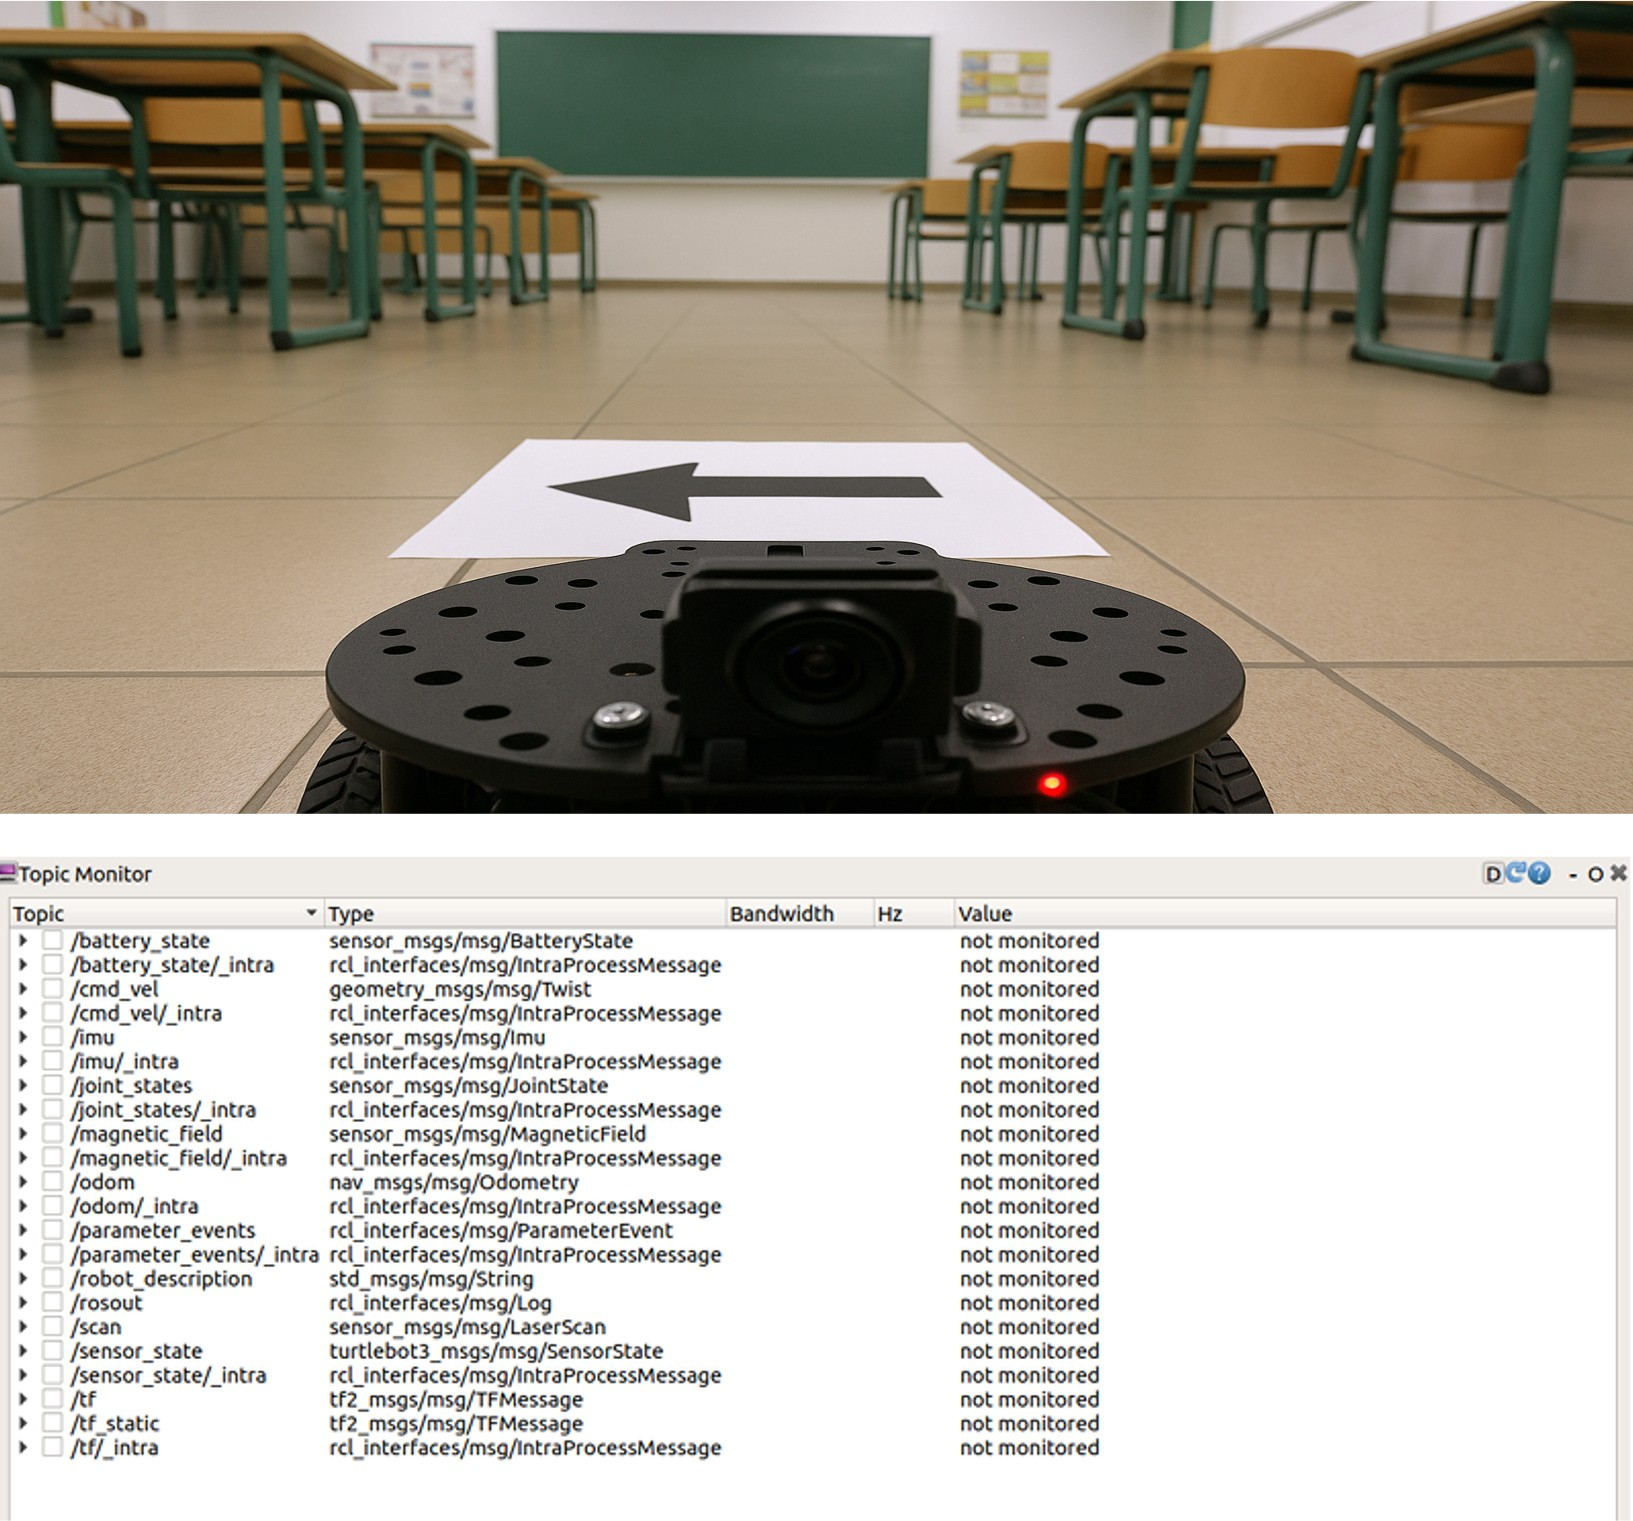
\includegraphics[width=\linewidth]{rqt}
    \caption{Topic-Monitor mit Image-View-Plugin (RQT)}\label{rqt}
\end{figure}
Im Rahmen der weiteren Einarbeitung wurde zudem die SLAM-Funktionalität (Simultaneous Localization and Mapping) getestet, um ein besseres Verständnis für die Navigation und Kartenerstellung mit dem TurtleBot3 in Kombination mit ROS 2 zu gewinnen. 
Diese ersten praktischen Erfahrungen bildeten die Grundlage für die darauf aufbauenden Entwicklungen im weiteren Projektverlauf.
\subsection{Einbinden der Kamera}
Der TurtleBot3 besitzt in seiner Standardausführung keine integrierte Kamera. 
Zu Beginn des Projekts war allerdings bereits eine externe Raspberry Pi Camera 1.3 nachgerüstet. 
Um diese korrekt in das System zu integrieren und mit ROS 2 nutzbar zu machen, waren mehrere Konfigurations- und Installationsschritte notwendig.
\newPar
Zunächst wurden auf dem Raspberry Pi alle erforderlichen Systempakete installiert, darunter \textit{libraspberrypi-bin}, \textit{v4l-utils} sowie das ROS-2-Paket \textit{ros-humble-v4l2-camera}, das die Nutzung von Kameras über das Video4Linux2-Interface ermöglicht. 
Zusätzlich wurde das Paket \textit{ros-humble-image-transport-plugins} installiert, um verschiedene Bildübertragungsformate (\zB~komprimierte Streams) in ROS~2 nutzen zu können. 
Damit der Benutzer auf die Kamera zugreifen darf, wurde dieser der Benutzergruppe \textit{video} hinzugefügt.
\newPar
Anschließend erfolgte die Konfiguration der Kamera über das Tool \textit{raspi-config}. 
Hierbei wurden im Menü unter \textit{Interface Options} sowohl die Legacy\hyp{}Kameraunterstützung als auch SPI und I2C aktiviert. 
Nach einem Systemneustart wurde mit dem Befehl \textit{vcgencmd get\_camera} überprüft, ob die Kamera korrekt erkannt wurde.
\newPar
Zum Start der Kamera in ROS 2 wurde schließlich der Node \textit{v4l2\_camera\_node} ausgeführt, wobei die gewünschte Auflösung von 640x480 Pixeln als Parameter übergeben wurde. 
Diese moderate Auflösung wurde gewählt, um ein flüssiges Videobild bei gleichzeitig geringer Systemauslastung sicherzustellen.
\subsection{Zusammenarbeit über Git}
Um im späteren Verlauf des Projekts eine parallele Entwicklung des Codes zu ermöglichen und einen einfachen Austausch zwischen den verwendeten Systemen sicherzustellen, wurde Git als Versionsverwaltungssystem eingesetzt. 
Zu diesem Zweck wurde ein zentrales Git-Repository eingerichtet, das der Projektgruppe eine strukturierte und nachvollziehbare Zusammenarbeit ermöglichte.
\newPar
Das Repository wurde in mehrere Branches unterteilt, um unterschiedliche Aufgabenbereiche klar zu trennen: 
Ein Branch diente der Projektdokumentation, ein weiterer dem späteren Training des YOLO-Modells, und ein dritter Branch wurde für die Implementierung der ROS 2-Nodes vorbereitet. 
Diese Aufteilung erleichterte nicht nur die Zusammenarbeit, sondern stellte auch sicher, dass Änderungen gezielt getestet und unabhängig voneinander weiterentwickelt werden konnten.
    \clearpage
    \section{Training des Modells}
Ein zentraler Bestandteil des Projekts ist das Training eines eigenen Objekterkennungsmodells auf Basis von YOLO. 
Da die vortrainierten Modelle keine spezifischen Erkennungsobjekte wie Richtungspfeile umfassen, ist es erforderlich, ein benutzerdefiniertes Modell zu trainieren. 
Ziel des Trainingsprozesses ist es, das Modell so anzupassen, dass es die gewünschten Objekte zuverlässig und in Echtzeit erkennen kann.
\subsection{Aufnahme der Trainingsbilder}
Ein zentraler Bestandteil beim Training eines eigenen Objekterkennungsmodells ist die Erstellung eines passenden Datensatzes. 
Dabei kommt es nicht nur auf die Anzahl der Bilder an, sondern auch auf deren Vielfalt. 
Ziel ist es, das Modell möglichst gut auf die realen Einsatzbedingungen vorzubereiten. 
Daher sollten die Trainingsbilder unterschiedliche Perspektiven, Lichtverhältnisse, Objektgrößen und -anordnungen abdecken. 
Je abwechslungsreicher die Bilder, desto robuster wird das Modell gegenüber späteren Anwendungsszenarien.
\cite{yolo_data_docu}
\newPar
Für dieses Projekt wurden die Trainingsdaten aufgenommen, indem verschiedene Pfeile in unterschiedlichen Farben und Formen ausgedruckt und im Raum verteilt wurden. 
Die Anordnung und Orientierung der Pfeile wurde dabei bewusst variiert, mit teilweise bis zu zehn Pfeile auf einem Bild.
Die Fotos wurden mit einem handelsüblichen Smartphone aufgenommen, wobei wir verschiedene Blickwinkel gewählt haben, um eine möglichst breite Datenbasis zu schaffen. 
Insgesamt wurden dabei mehrere hundert Bilder erzeugt, in denen zusammen ca. tausend Pfeile zu sehen sind.
Diese Daten dienen als Grundlage für das nachfolgende Training des Modells.
\subsection{Vorverarbeitung und Labeling}
Für das Training von Objekterkennungsmodellen wie YOLO ist die Bildgröße ein wichtiger Faktor.
Modelle dieser Art erwarten in der Regel Eingabebilder mit festen Abmessungen, da neuronale Netze mit gleichbleibender Eingabegröße arbeiten.
\newPar
Im Projekt wurde sich für die Größe 640 x 480 Pixel entschieden, da mit entsprechend höherer Bildgröße auch der Speicher- und insbesondere der Rechenbedarf steigt.
Auch bei der Inferenz, also dem späteren Einsatz des trainierten Modells zur Objekterkennung, ist eine einheitliche Bildgröße erforderlich.
Die Eingabebilder werden dabei entweder im Vorfeld oder automatisch vom System auf die vom Modell erwartete Größe skaliert.
Es ist daher sinnvoll, die Bilder bereits vor oder während der Vorbereitung des Trainingsdatensatzes in das gewünschte Format zu bringen.
Als Vorverarbeitung der Traingsdaten wurden die Bilder daher auf eine Größe von 640 x 480 Pixel runterskaliert.
Dadurch konnte die Trainingszeit verkürzt und der Speicherbedarf reduziert werden. 
Ein Beispiel Trainingsbild ist in \imageref{beispiel_trainingsbild} dargestellt.
\cite{yolo_pre_docu}
\begin{figure}[H]
    \centering
    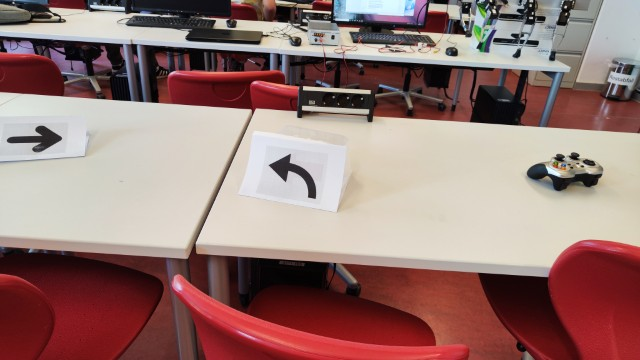
\includegraphics[width=0.75\linewidth]{example_image}
    \caption{Beispiel Trainings-Bild \textit{4f7e6590-88.jpg}}\label{beispiel_trainingsbild}
\end{figure}
Für den fertigen Trainings\hyp{}Datensatz wird zusätzlich zu den Bildern auch die dazugehörige Annotationsdatei benötigt. 
Diese enthalten Informationen über die Position und Klasse der Objekte im Bild, üblicherweise im sogenannten YOLO-Format.
Dieses speichert die Informationen in zwei Dateien, die jeweils den gleichen Dateinamen mit unterschiedlicher Endung aufweisen.
Das Bild an sich hat die entsprechende Bildformat-Endung, wie .jpg oder .png. Zusätzlich existiert eine Datei mit der Endung .txt, welche die Annotationen enthalten.
\cite{yolo_format_docu}
\newPar
Die zum Trainingsbild zugehörige Annotationsdatei \textit{4f7e6590-88.txt} sieht folgendermaßen aus:
\begin{lstlisting}
1 0.0552519011406844 0.3852978453738909
        0.09767110266159694 0.08365019011406837
0 0.4708606114138901 0.4680150843996924
        0.09415121255349486 0.1597717546362342
\end{lstlisting}

Dabei gibt die erste Zahl jeder Zeile die Klasse des Objektes und die nachfolgenden die Koordinaten der Bounding Box an.
\cite{yolo_format_docu}
\begin{figure}[H]
    \centering
    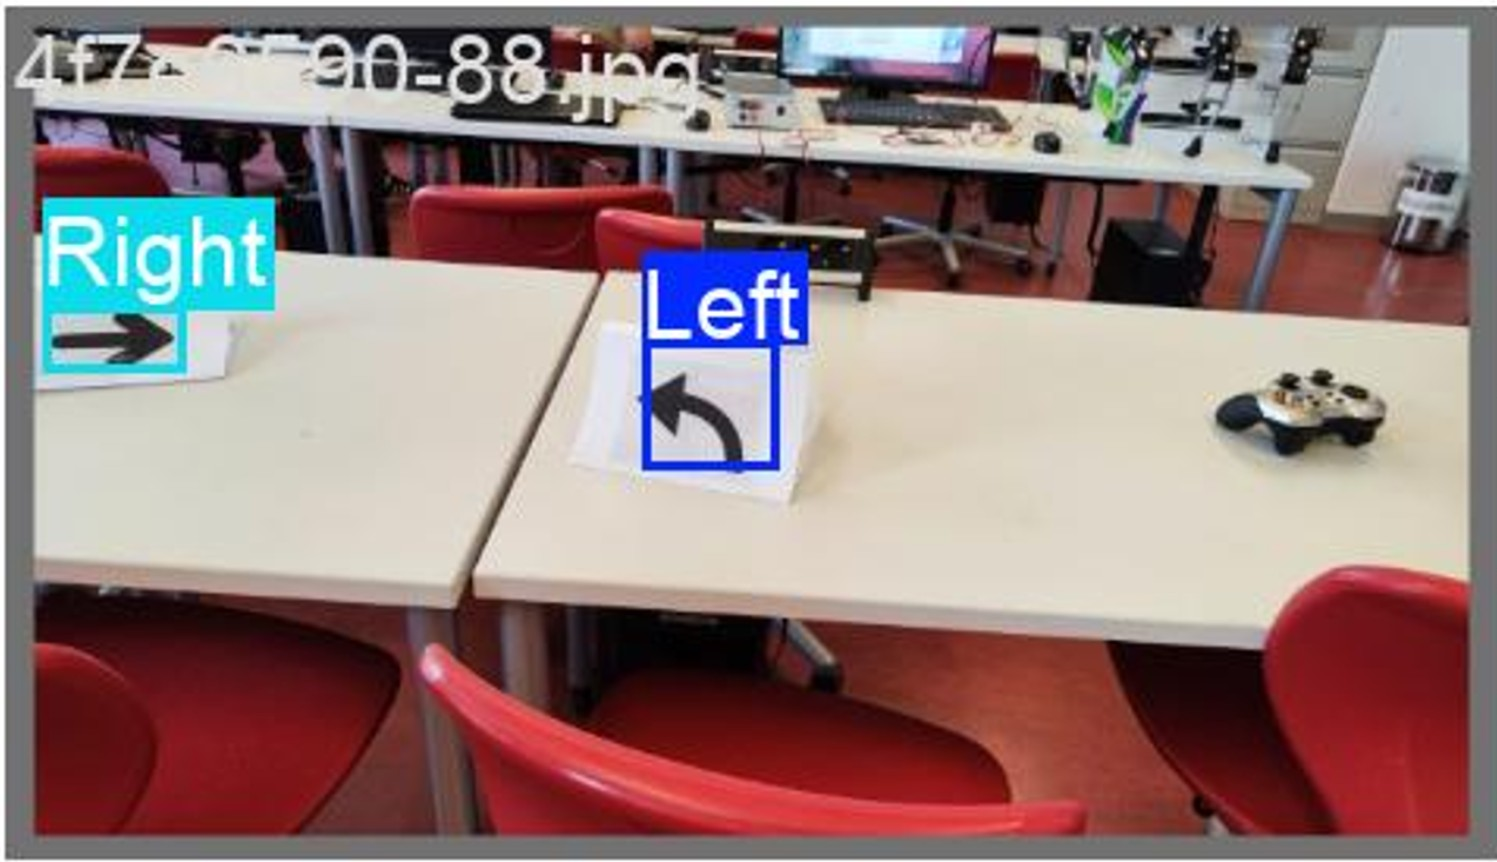
\includegraphics[width=0.8\linewidth]{example_labled}
    \caption{Beispiel gelabeltes Trainings-Bild}\label{beispiel_trainingsbild_labeld}
\end{figure}
Zusammengeführt sieht dieses Labelling dann entsprechend \imageref{beispiel_trainingsbild_labeld} aus.
Die Annotation der Daten kann mit speziellen Tools durchgeführt werden.
Im Projekt wurde dazu das Tool \gq{LabelStudio} von HumanSignal eingesetzt. Dieses stellt ein einfaches Web-Interface bereit, in dem das Labelling komfortabel vorgenommen werden kann.
\cite{labelstudio}
\subsection{Training}
Neben dem Datensatz selbst wird auch eine passende Trainingsumgebung benötigt. Dazu gehört Python als Programmiersprache sowie die Bibliothek PyTorch. 
Das eigentliche Training sollte mithilfe einer GPU erfolgen, da die Rechenprozesse sehr aufwendig sein können. Wichtig ist außerdem die Konfiguration des Modells und des Trainingsprozesses. 
Hierzu zählen unter anderem die Definition der Objektklassen und die Anzahl der Trainingsdurchläufe (Epochen).
\newPar
Für das Training des Modells wurde der aufbereitete Datensatz zunächst in Trainings\hyp{} und Validierungsdaten aufgeteilt. 
Dabei wurde ein klassisches 80/20\hyp{}Verhältnis gewählt, also 80\% der Bilder für das eigentliche Training und 20\% zur Validierung. 
Der Sinn dieser Aufteilung liegt darin, die Leistung des Modells nicht nur auf den gelernten Trainingsdaten zu beurteilen, sondern auch auf bisher \gq{unbekannten} Daten, 
um eine Überanpassung (das sogenannte Overfitting) zu vermeiden. 
Während des Trainings wird die Modellleistung regelmäßig mit den Validierungsdaten überprüft, wodurch die Modellqualität und der Lernfortschritt beurteilt werden kann.
\newPar
Das Training selbst wurde auf einem Laborrechner mit einer NVIDIA RTX 4060 Ti in der 16GB Variante durchgeführt. Es wurde keine feste Anzahl an Epochen vorgegeben. 
Stattdessen kam ein sogenanntes Early-Stopping-Verfahren zum Einsatz. Dabei wird das Training automatisch beendet, 
sobald sich die Modellleistung über einen bestimmten Zeitraum nicht mehr verbessert hat.
Dies wird, wie oben erläutert, anhand der Validierungsdaten gemessen. Im konkreten Fall wurde das Training nach etwa 300 Epochen abgebrochen. 
Eine Epoche dauerte durchschnittlich rund 800 Millisekunden, was zu einer Gesamttrainingszeit von etwa vier Minuten führte.
\newPar
Zum Vergleich: Ein Testlauf auf der virtuellen Maschine ohne GPU, also mit reinem CPU-Training, benötigte für das gleiche Training durch die deutlich schlechtere Performance und 
längere Reaktionszeit pro Epoche über eine Stunde. Dieser Vergleich unterstreicht den großen Einfluss der verwendeten Hardware auf die Effizienz und Praktikabilität des Trainingsprozesses. 
Besonders bei größeren Datensätzen oder komplexeren Modellen ist eine GPU-Unterstützung nahezu unerlässlich.
\newPar
An diesem Punkt wurde daher entschieden, die Inferenz und die Steuerung des Roboters aus Performancegründen auch auf den Laborrechner zu verschieben.
\subsection{Bewertung}
Zur Beurteilung des Modells können mehrere von PyTorch generierte Metriken betrachtet werden. Einen sehr guten, schnellen und einfach verständlichen Überblick bietet die sogenannte
Confusion-Matrix in \imageref{conf_matr} (hier in normalisierter Form).

\begin{figure}[H]
    \centering
    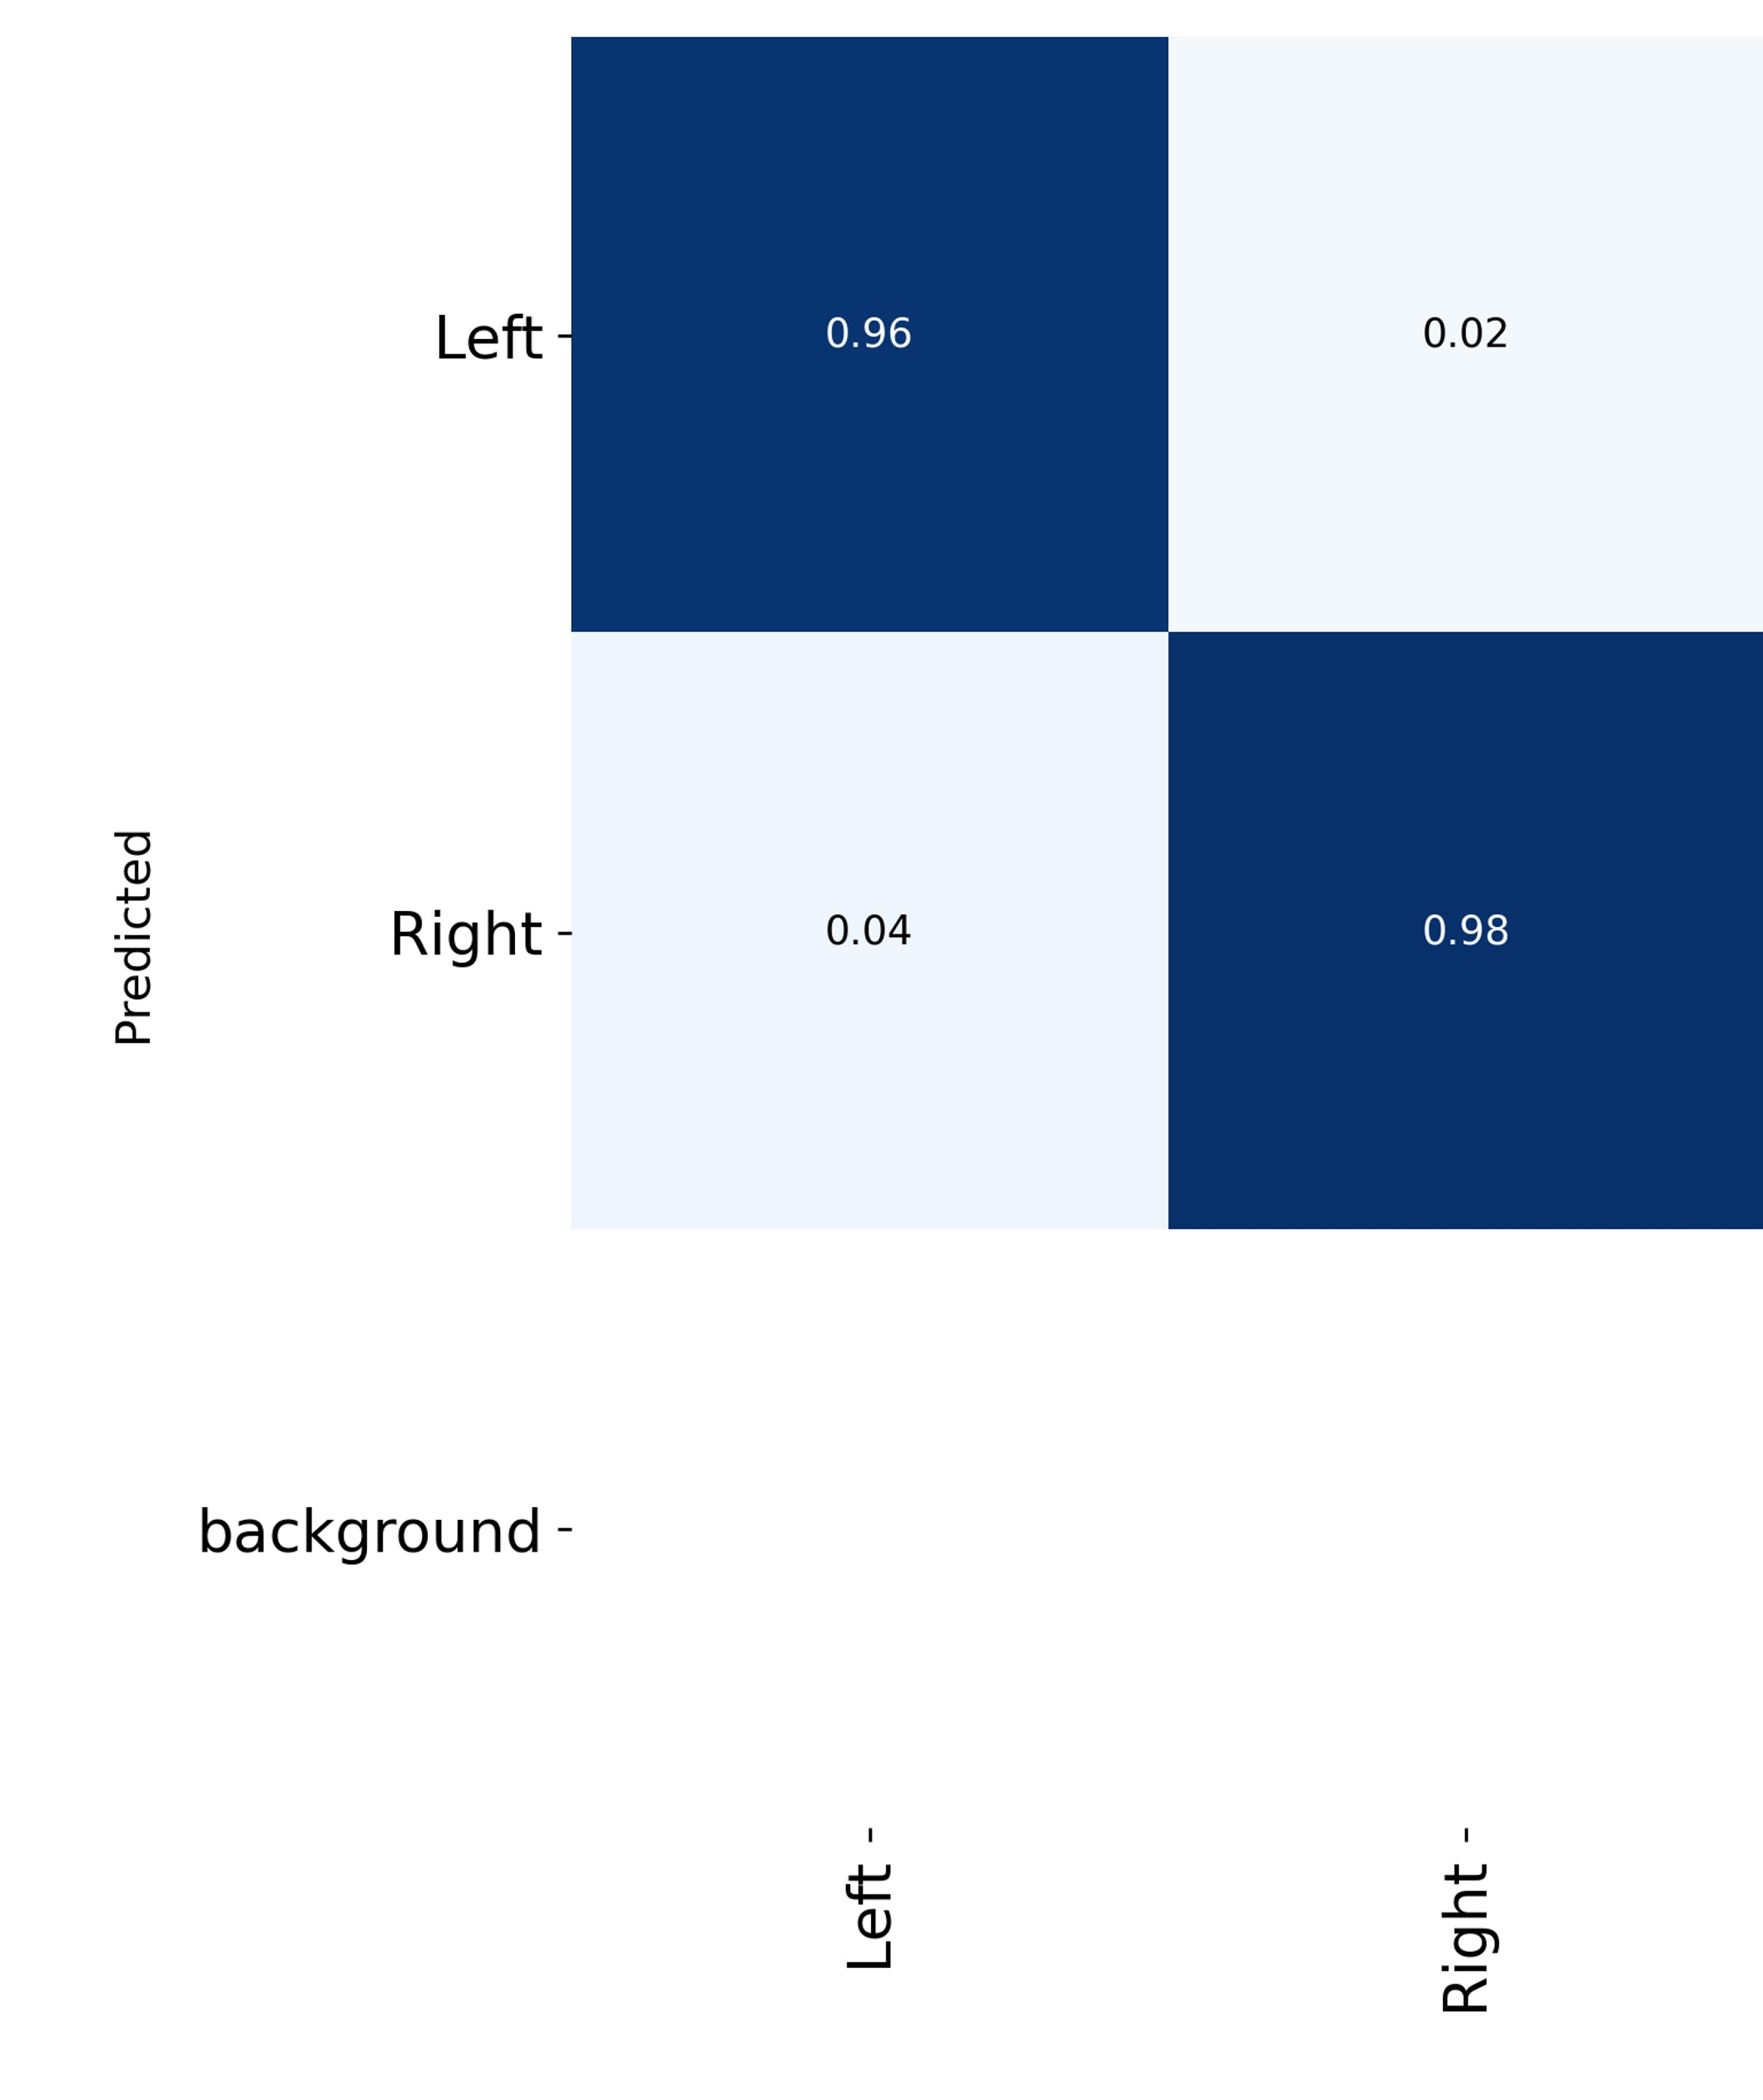
\includegraphics[width=0.7\linewidth]{conf_matr}
    \caption{Normalisierte Confusion-Matrix des Trainings}\label{conf_matr}
\end{figure}

Dabei sind auf der X-Achse die gelabelten Bounding Boxen und auf der Y-Achse die erkannten Bounding Boxen (predictions) der Klassen aufgetragen.
Hier können Korrelationen der Klassen beziehungsweise problematische Konfusionen erkannt werden.
\cite{yolo_metrics}
\newPar
Dem speziellen Beispiel kann beispielsweise entnommen werden, dass 96\% der als \textit{Left} gelabelten Objekte und 98\% der als \textit{Right}
gelabelten Objekte auch als solche erkannt werden.
\newPar
Umfangreichere Einblicke in den Trainingsvorgang sowie die \hyp{}qualität bietet die Ergebnisübersicht.

\begin{figure}[H]
    \centering
    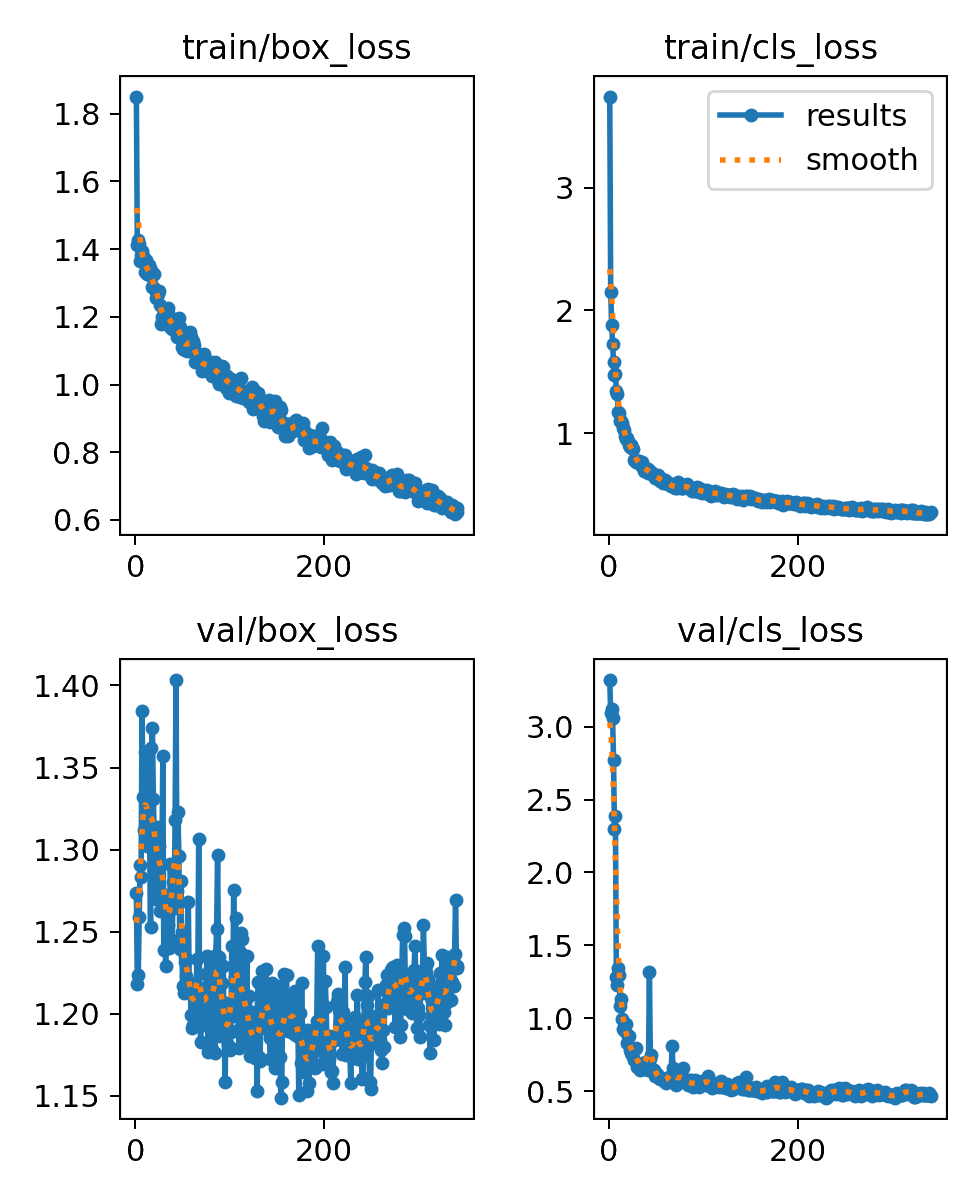
\includegraphics[width=0.6\linewidth]{results}
    \caption{Auschnitt der Ergebnisübersicht des Trainings}\label{results}
\end{figure}

Die in \imageref{results} dargestellten Graphen zum Box-Loss \textit{box\_loss} und zum Klassifikationsverlust \textit{cls\_loss} zeigen den Verlauf dieser beiden zentralen Fehlerfunktionen während des Trainings 
und der Validierung des Modells über die etwa 300 Epochen des Trainings. Die obere Reihe bezieht sich dabei auf die Trainings\hyp{} und die untere auf die Validierungsdaten.
Beide Diagramme erlauben Rückschlüsse auf die Lernfortschritte des Modells und dessen Fähigkeit, die Trainingsdaten korrekt zu verarbeiten und auf unbekannte Daten anzuwenden.
\newPar
Beim Box-Loss handelt es sich um den Fehler, den das Modell bei der Vorhersage der Position und Größe der Objekte macht. 
Im Trainingsverlauf ist ein klarer Rückgang des Box-Loss-Werts von anfangs etwa 1,8 auf unter 0,7 erkennbar. 
Dies deutet darauf hin, dass das Modell zunehmend lernt, die Objekte räumlich korrekt zu lokalisieren. 
Die Abnahme erfolgt kontinuierlich und ohne größere Schwankungen, was für ein stabiles Lernverhalten spricht. 
Im Validierungsdiagramm ist zunächst ebenfalls ein Rückgang zu erkennen, gefolgt von einem leichten Anstieg gegen Ende des Trainings. 
Dieser Verlauf kann ein Hinweis darauf sein, dass das Modell beginnt, sich zu stark an die Trainingsdaten anzupassen.
Also das oben bereits erwähnte sogenannte Overfitting.
\newPar
Der Klassifikationsverlust (\textit{cls\_loss}) beschreibt, wie gut das Modell die erkannten Objekte der richtigen Klasse zuordnet. 
Auch hier zeigt sich im Trainingsverlauf ein starker Rückgang des Fehlers, insbesondere in den frühen Epochen, gefolgt von einer langsamen Annäherung an einen stabilen Wert um 0,6. 
Das bedeutet, dass das Modell sehr schnell die grundlegenden Klassifizierungsregeln erlernt und sich dann zunehmend feiner an die Daten anpasst. 
Auf dem Validierungsdatensatz ist dieser Trend ebenfalls sichtbar, jedoch mit stärkeren Schwankungen. 
Trotzdem bleibt der Verlauf weitgehend stabil, was auf eine solide Inferenz des Modells schließen lässt.
\cite{yolo_metrics}
\newPar
Insgesamt zeigen beide Metriken, dass das Modell im Training effektiv lernt. 
Die klare Abnahme der Verluste und das weitgehend parallele Verhalten auf Trainings- und Validierungsdaten sprechen für einen erfolgreichen Optimierungsprozess, 
auch wenn sich gegen Ende eine mögliche Überanpassung andeutet.
    \section{Implementierung}
Nachdem alle vorbereitenden Maßnahmen abgeschlossen und die Systemkomponenten erfolgreich konfiguriert worden sind, begann die eigentliche Implementierungsphase des Projekts. 
Ziel war es, einen eigenen ROS-2-Node zu entwickeln, der die Bilddaten der Kamera verarbeitet, das trainierte Modell zur Objekterkennung nutzt und den Roboter entsprechend steuert.
Im Folgenden wird die schrittweise Erstellung und Integration dieses Nodes beschrieben.
\subsection{Anlegen eines neuen ROS Package}
Für die Verarbeitung der Bilddaten wurde ein neues ROS-2-Paket in Python erstellt. 
Dabei kam das Build-System \textit{ament} zum Einsatz, das in ROS 2 als Standard für die Verwaltung und den Aufbau von Paketen dient. 
Es ermöglicht eine klare Strukturierung des Codes und unterstützt die einfache Integration von Abhängigkeiten und Erweiterungen. 
Im Rahmen der Paketerstellung wurde ein Node mit dem Namen \textit{camera\_stream} angelegt, der als Grundlage für die spätere Bildverarbeitung dient.
\newPar
Nach dem Anlegen des Pakets erfolgte eine erstmalige Kompilierung und Registrierung im ROS-2-Workspace. 
Durch das Aktualisieren der Entwicklungsumgebung konnte sichergestellt werden, dass das neue Paket korrekt erkannt und ausgeführt werden kann.
\subsection{Auslesen der Kamera}
Die Bilddaten werden mittels eines ROS-2-Subscribers empfangen, der das Topic \textit{/image\_raw/compressed} abonniert. 
Dieses Topic stellt die komprimierten Bilder der Raspberry Pi Kamera über den bereits erwähnte \textit{v4l2\_camera}-Node bereit. 
Im Callback der Subscription werden die eingehenden Daten in einem Buffer zwischengespeichert.
\newPar
Die empfangenen Bilddaten werden mit OpenCV aus dem komprimierten Format decodiert und anschließend gespiegelt, um die Kameraperspektive korrekt abzubilden.
Dies ist notwendig, da die Kamera um 180° gedreht montiert wurde.
Die so vorbereiteten Frames werden kontinuierlich für die anschließende Objekterkennung bereitgestellt.
\subsection{Aufruf des trainierten YOLO-Modells}
Für die Objekterkennung wird das trainierte YOLO-Modell verwendet, das mithilfe der Ultralytics-Bibliothek in den ROS-Node integriert eingebunden wurde. 
Nach Initialisierung des Modells und Prüfung der CUDA-Verfügbarkeit zur optionalen GPU-Beschleunigung werden Bilddaten mit einer festen Auflösung von 640x480 Pixeln als Eingabe verarbeitet.
\newPar
Die Inferenz des Models wird synchron ausgeführt und liefert eine Liste von erkannten Objekten mit zugehörigen Klassen und Konfidenzwerten. 
Eine Konfidenzschwelle von 0,7 filtert unsichere Erkennungen aus. 
Bei mehreren Erkannten Objekten, wird immer das Objekt mit dem höchsten Konfidenzwert ausgewertet.
Die Erkennungsergebnisse werden für die Steuerlogik genutzt und zur Visualisierung als Overlay in das Bild eingefügt.
Die Visualisierung des aktuellen Bilds erfolgt mit OpenCV.
Somit hat man während der Ausführung der Node einen Videostream mit den aktuell Erkannten Objekten als Overlay.
\subsection{Steuerung des TurtleBot3}
Die Bewegungssteuerung des TurtleBot3 erfolgt über einen ROS 2 Publisher, der Bewegungsbefehle auf dem Topic \textit{cmd\_vel} publiziert. 
Zur Umsetzung der Fahrbefehle werden vordefinierte lineare und Winkel\hyp{}Geschwindigkeiten verwendet, die ca. der Hälfte der Maximalgeschwindigkeit des Turtlebot entsprechen. 
\newPar
Die Steuerlogik wertet über eine Hysterese, d.\,h. eine Schwellenwertlogik, die Häufigkeit der erkannten Richtungspfeile (\gq{Left} bzw. \gq{Right}) aus mehreren aufeinanderfolgenden Bildern aus. 
Erst wenn eine Richtung ausreichend oft detektiert wurde, erfolgt die entsprechende Bewegungsanweisung zum Abbiegen. 
Andernfalls fährt der Roboter geradeaus.
Durch diese Hysterese wird eine stabile und verwacklungsfreie Steuerung gewährleistet, da einzelne Fehlinterpretationen durch die Aggregation über mehrere Bilder ausgeglichen werden. 

    \section{Zusammenfassung}
Im Rahmen dieses Projekts wurde ein System zur Echtzeit-Bilderkennung und autonomen Steuerung eines mobilen Roboters entwickelt. 
Dabei kamen sowohl moderne Deep-Learning-Technologien als auch bewährte Frameworks aus der Robotik zum Einsatz. 
In diesem Kapitel werden abschließend aufgetretene Herausforderungen beleuchtet sowie Ansätze für mögliche Verbesserungen aufgezeigt.
\subsection{Herausforderungen während des Projekts}
Im Verlauf des Projekts traten verschiedene Herausforderungen auf, die sowohl das Modelltraining als auch die Integration der Lösung betrafen. 
Zu Beginn stand eine zu geringe Anzahl an Trainingsbildern zur Verfügung, was sich deutlich in der schlechten Erkennungsleistung der ersten Traingsversuche zeigte. 
Erst durch die Erweiterung des Datensatzes mit deutlich mehr Bildern konnte eine brauchbare Modellqualität erreicht werden. 
\newPar
Zusätzlich gestaltete sich die Integration des Raspberry Pi und der VM als aufwendig, da eine funktionierende Netzwerk- und VM-Konfiguration erforderlich war, 
um eine stabile Kommunikation zwischen dem Raspberry und der Virtuellen Maschine sicherzustellen. 
\newPar
Softwareseitig gab es die Herausforderung, auf dem eingesetzten Ubuntu-System des Raspberry Pi einige notwendige Pakete und Treiber zu installieren.
So war beispielsweise nur die Kamera-Version 1.3 verwendbar, da neuere Modelle oder die Nutzung mit Tools wie GStreamer mangels Treiberunterstützung nicht funktionierten. 

\subsection{Ansätze für die Verbesserung}
Im Verlauf der Arbeit ergaben sich auch einige wichtige Erkenntnisse und mögliche Verbesserungsansätze für zukünftige Projekte. 
Eine davon ist der Einsatz von sogenannten Oriented Bounding Boxes, also gedrehten Boxes, die neben Position und Größe auch die Orientierung eines Objekts erfassen. 
Gerade bei der Erkennung von Pfeilen kann dadurch nicht nur das Objekt selbst, sondern auch dessen Richtung eindeutig erkannt werden.
\cite{yolo_obb}
Das würde Fehler vermeiden, bei denen ähnlich aussehende, aber entgegengesetzt ausgerichtete Pfeile verwechselt wurden. 
Allerdings ist dabei das Labelling deutlich aufwendiger, da neben den üblichen Informationen auch der Rotationswinkel manuell erfasst werden muss. 
\newPar
Eine weitere Erkenntnis betrifft den Einsatz von sogenannten Background Images, also Bildern ohne relevante Objekte. 
Solche Bilder helfen dem Modell dabei zu lehren, dass nicht in jedem Bild zwingend ein Pfeil vorhanden ist. 
Dadurch lassen sich False Positives reduzieren, also Fehler, bei denen das Modell fälschlicherweise ein Objekt erkennt
\newPar
Beide Ansätze tragen dazu bei, die Genauigkeit und Zuverlässigkeit des Modells in realen Anwendungen weiter zu verbessern.

\subsection{Repository}
Das GIT-Repository dieses Projektes ist auf GitHub unter folgendem Link zu finden: https://github.com/SchaeferDa/AMR.
    \newpage
    \newpage
    \bibliography{literatur}
    % \bibliographystyle{apalike}
    \bibliographystyle{ieeetran}
    \newpage
    \listoffigures
    %\listoftables
\end{document}
